\section{Model Repair for Resiliency}
\seclabel{result}
%\vspace{-0.5em}
%
%
In this section, we demonstrate the capability of \toolreaffirm to repair CPSs models under unanticipated attacks. We first revisit the ACC model and evaluate more resilient patterns that can be applied to repair the model under the GPS sensor attack. Second, we investigate a sliding-mode switching attack that causes instability for a smart grid system, and how \toolreaffirm can be applied to automatically repair the model under this attack.

\subsection{Adaptive Cruise Control System}
{\bf GPS Sensor Attack Construction.} To perform a spoofing attack on the GPS sensor of the ACC model, we continuously inject a false data to manipulate its measurement value. In this case, we omit the original assumption $|\ngps| \leq 0.05$, and employ the new assumption as $|\ngps| \leq 50$. Using the input generator in Breach, we specify the GPS spoofing attack as a standard input test signal such as a constant, ramp, step, sinusoid or random signal whose amplitude varies over the range of [-50, 50]. 


\vspace{0.5em}
\noindent
{\bf Additional Resilient Patterns for ACC model.} Under the GPS spoofing  attack, the original ACC model does not satisfy its safety requirement and a designer needs to apply a certain resilient pattern to repair the model. The first example of such a resilient pattern for the ACC model have been introduced in~\secref{overview}, which makes a resilient copy of the original model where the controller simple ignores the GPS reading as it can no longer be trusted. However, we need to determine the best switching condition from the original model to the resilient copy.~\figref{acc_model_pat1} shows the completed, resilient model in which the switching condition is determined by synthesizing the value of $\theta$ using Breach. In the attack scenario, we assume that the GPS spoofing occurs at every time point, specified as a random constant signal over the range of [-50, 50].   

\begin{figure}[t!]%
	\centering%
    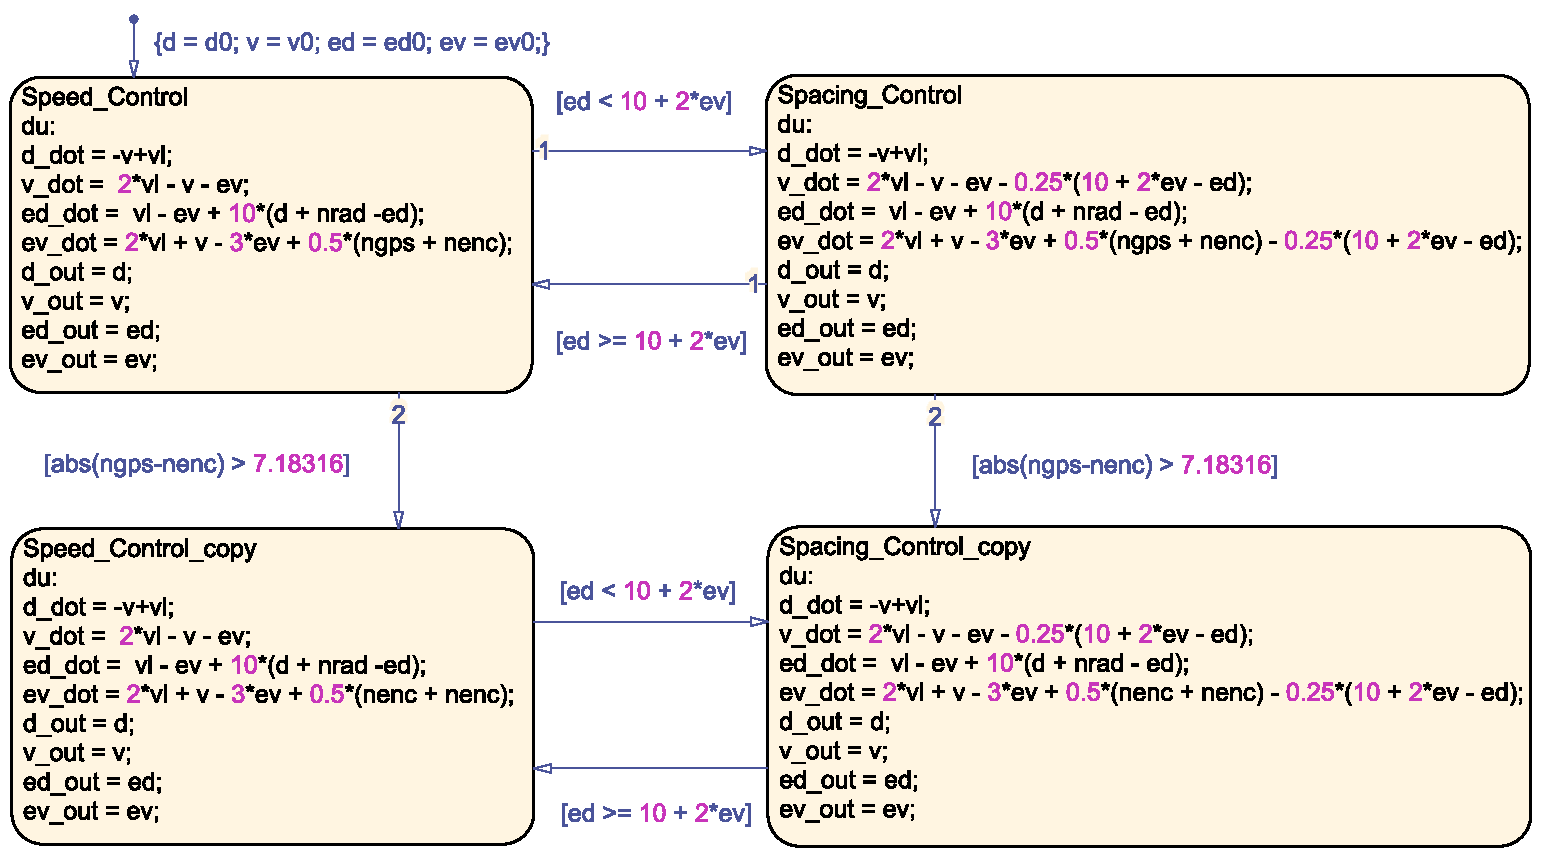
\includegraphics[width=0.48\textwidth]{image/acc_model_pat1}%\vspace{1cm}
		%\includegraphics[trim = 17mm 85mm 17mm 0mm, clip, width=0.95\textwidth]{image/spectral_signal}%
	\caption{the resilient ACC model with a synthesized value of $\theta = 7.18316$.}%
	\figlabel{acc_model_pat1}%
\end{figure}% 

The second resilient pattern is an extended version of the first one by specifying a switching-back condition from the resilient copy to the original model when the GPS sensor is detected and mitigated. An example of such a switching-back condition is when the difference between the $\nenc$ and $\ngps$ are getting smaller, \ie $|\ngps -\nenc| < \theta - \epsilon$, where $\epsilon$ is a positive user-defined tolerant. For this pattern, the model transformation script can be written similar to the one shown in~\figref{examplecode} with adding the \emph{addTransition} function from the copy mode to the original mode with the guard condition labeled as $|\ngps -\nenc| < \theta - \epsilon$ in the \emph{formode} loop.



Alternatively, another resilient pattern, which we do not need to modify the structure of the original model, is to model the redundancy in the sensory information as a linear combination of different sensor measurements. For example, instead of taking the average of $\ngps$ and $\nenc$, we can model their relationship as $\theta\ngps + (1-\theta)\nenc$, and then synthesize the value of $\theta$ so that the safety property is satisfied. The transformation script of this resilient pattern is given in~\figref{acc_code_3}. For this pattern, we assume that a designer still wants to use all sensor measurements even some of them are under spoofing attacks and would like to search for the value of $\theta$ over the range of [0.2, 0.8] (instead of [0, 1]). Given the same attack model for the other patterns, the synthesizer in \toolreaffirm fails to find the value of $\theta$ within the given range to ensure the safety property holds. However, if we enlarge the range of $\theta$ to [0.1, 0.9], the synthesizer successfully find the safe value $\theta = 0.1543$, and the resilient model shown in~\figref{acc_model_pat3}. 
%
This result indicates that the pattern can repair the model if the GPS spoofing attack specified over a small range, but will fail for a larger range (\eg $|\nenc| \leq 100$).           

\begin{figure}[!t]%frame=none,
\begin{lstlisting}[basicstyle=\ttfamily\footnotesize, numbers=none]
model = getModelByName("ACC") # retrieve the ACC model

# start a transformation  
formode m = model.Mode {
    replace(m.flow,"ngps", "2*theta*ngps")
    replace(m.flow,"nenc", "2*(1-theta)*nenc")
}
# end of the transformation
\end{lstlisting}
\caption{The third resilient pattern for the ACC system based on the linear combination of $\nenc$ and $\ngps$.}%
\figlabel{acc_code_3}%
	%\vspace{-0.5em}%
\end{figure}


\begin{figure}[t!]%
	\centering%
    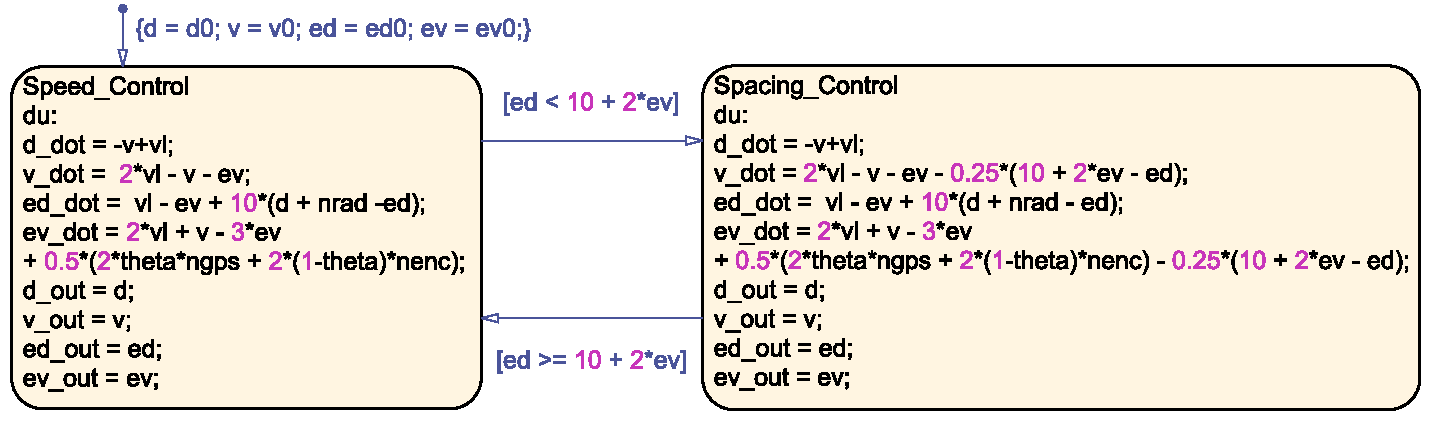
\includegraphics[width=0.48\textwidth]{image/acc_model_pat3}%\vspace{1cm}
		%\includegraphics[trim = 17mm 85mm 17mm 0mm, clip, width=0.95\textwidth]{image/spectral_signal}%
	\caption{the resilient ACC model with a synthesized value of $\theta = 0.1543$ for the resilient pattern shown in ~\figref{acc_code_3}.}%
	\figlabel{acc_model_pat3}%
\end{figure}% 




\subsection{Single-Machine Infinite-Bus System}
%

\begin{figure}[t!]%
	\centering%
    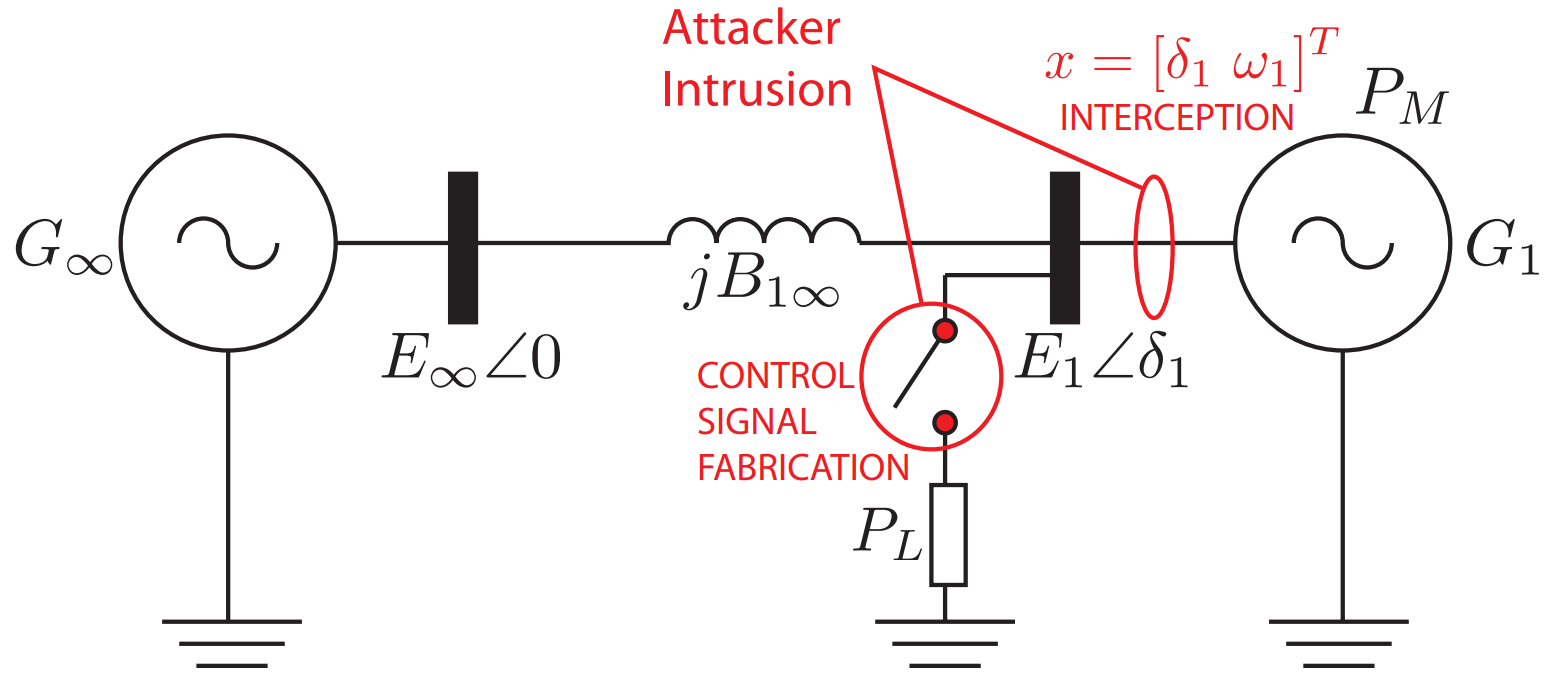
\includegraphics[width=0.42\textwidth]{image/smib}%
		%\includegraphics[trim = 17mm 85mm 17mm 0mm, clip, width=0.95\textwidth]{image/spectral_signal}%
	\caption{Single-machine infinite-bus model~\cite{farraj2014practical}.}%
	\figlabel{smib}%
\end{figure}%

Next, we study a class of cyber-physical switching attacks that can destabilize a smart grid system model, and then apply \toolreaffirm to repair the model to provide resilience. 

\vspace{0.5em}
\noindent
{\bf Original SMIB Model.}
A smart power grid system such as the Western Electricity Coordinating
Council (WECC) 3-machine, 9-bus system~\cite{sauer1998power}, can be represented as a single-machine infinite-bus (SMIB) model shown in~\figref{smib}\footnote{the figure is copied from \cite{farraj2014practical}.}. In this model, $G_\infty$ and $G_1$ correspondingly represent the SMIB and local generators; $B_\infty$ and $B_1$ denote the infinite and local bus, respectively; $E_\infty$ is the infinite bus voltage; $E_1$ is the internal voltage of $G_1$; $B_{1\infty}$ is the transfer susceptance of the line between $B_1$ and $B_\infty$; and $P_M$ is the mechanical power of $G_1$. The local load $P_L$ is connected or disconnected to the grid by changing a circuit breaker status. 
%
The SMIB system is considered as a \emph{switched system} in which the physical dynamics are changed between two operation modes based on the position of the circuit breaker. 
%
%
For an appropriate selection of parameters~\cite{farraj2014practical}, the second-order swing equation which characterizes the transient stability of the local generator $G_1$ can be described as:
%
\begin{align}
\dot{\delta_1} & = \omega \nonumber \\
\dot{\omega} & = 
\begin{cases}
    -10sin\delta_1 - \omega_1, & \text{if $P_L$ is connected}.\\
    9 - 10sin\delta_1 - \omega_1, & \text{if $P_L$ is disconnected},
 \end{cases} \nonumber
\end{align}
%
where, $\delta_1$, $\omega_1$ are the deviation of the rotor angle and speed of $G_1$ respectively, and $x = [\delta_1,\omega_1]^T$ is the state vector of $G_1$.
%
%

The swing equation of the SMIB system shown above has an interesting property known as a \emph{sliding mode} behavior. This behavior occurs when the state of the system is attracted and subsequently stays within the \emph{sliding surface} defined by a state-dependent switching signal $s(x)\in\Real$~\cite{decarlo1988variable, liu2014coordinated}. An example of a sliding surface is $s(x) = 0$. When the system is confined on a sliding mode surface, its dynamics exhibit high-frequency oscillations behaviors, so-called a \emph{chattering} phenomenon, which is well-known in the power system design~\cite{sabanovic2004variable}.
%
At this moment, if the attacker conducts the fast switchings between two  operation modes, the system will be steered out of its desirable equilibrium position. As a result, the power system becomes unstable even if each individual subsystem is stable~\cite{liu2014coordinated}.  
% 

\vspace{0.5em}
\noindent
{\bf Sliding-mode Attack Construction.} To successfully perform sliding-mode attack to a power grid system, we assume that the attack can a) gain some knowledge about the state information to mathematically construct an unstable sliding surface that can destabilize the system, and b) access to the communication channel to control the circuit breaker position. We note that a sliding-mode attack can be considered as a cyber-physical attack as it manipulate on both physical and cyber parts of the system. For the SMIB model with the swing equation defined previously, an attacker can use a sliding surface $s(x) = \delta_1 + \omega_1$ to calculate the value of the switching signal based on the following equation.
%
\begin{align}
\dot{\delta_1} & = \omega \nonumber \\
\dot{\omega} & = 
\begin{cases}
    -10sin\delta_1 - \omega_1, & \text{$s(x) \geq \epsilon$}.\\
    9 - 10sin\delta_1 - \omega_1, & \text{$s(x) < -\epsilon$},
 \end{cases} \nonumber
\end{align},
where $\epsilon$ represents switching delays and hysteresis~\cite{liu2011class}.
%

The stages of sliding-mode attack can summarized as follows.
\begin{enumerate}
	\item The attacker switches the circuit breaker to connect the load to the grid,
	\item when $\delta_1 + \omega_1 < -\epsilon$, the attacker switches the circuit breaker to disconnect the load, 
  \item when $\delta_1 + \omega_1 \geq \epsilon$, the attacker switches the circuit breaker to connect the load,
  \item the attacker repeats steps (1) and (2) until the system is driven out of the stability boundary, and then
  \item permanently switches the circuit breaker to disconnect the load.
\end{enumerate}
%
In this paper, we model the sliding-mode attack to the SMIB model as a Simulink/Stateflow diagram including two Stateflow models, where the plant model displayed in \figref{smib_plant_model} represents the physical dynamics of the system and the attack model is shown in \figref{smib_attack_model}. 
%
In the plant model, $\delta_1$ and $\omega_1$ are represented by $delta$ and $omega$, respectively; and the initial conditions are $delta0 \in [0, 1.1198]$ and $omega0 \in [0, 1]$. The discrete variable $load$ captures the open and closed status of the circuit breaker.
%
In the attack model, the attacker selects $\epsilon = 0.2$, and the local variable $t$ captures a simulation duration. We note that two transitions from the first mode to the second mode are executed with priorities such that the load is permanently disconnected at some instance where $t \geq 2.5$ seconds. 
%
%
\figref{smib_result} illustrates the examples of stable (\ie without an attack) and unstable (\ie a counterexample appearing under the sliding-model attack) behaviors of the SMIB system returned by running the falsifier of Breach, respectively. The red box defines the stable (safe) operation region of the SMIB that can be formalized as the following STL formula, 
%
\begin{align} 
\vspace{-1em}
	\varphi_{smib} & = \Box_{[0, T]} (0 \leq \delta_1[t] \leq 3.5) \wedge (-2 \leq \omega_1[t] \leq 3),\formlabel{smib_stl}
\end{align} 
where $T$ is a simulation duration.   
%
\begin{figure}[t!]%
	\centering%
    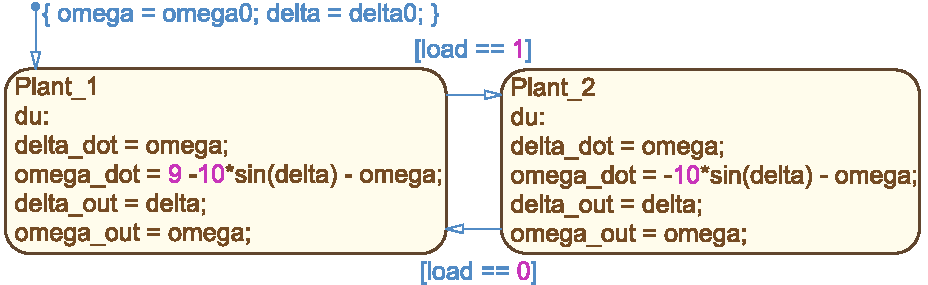
\includegraphics[width=0.48\textwidth]{image/smib_plant_model}%\vspace{1cm}
		%\includegraphics[trim = 17mm 85mm 17mm 0mm, clip, width=0.95\textwidth]{image/spectral_signal}%
	\caption{The Stateflow chart models the plant of the SMIB system.}%
	\figlabel{smib_plant_model}%
\end{figure}% 

\begin{figure}[t!]%
	\centering%
    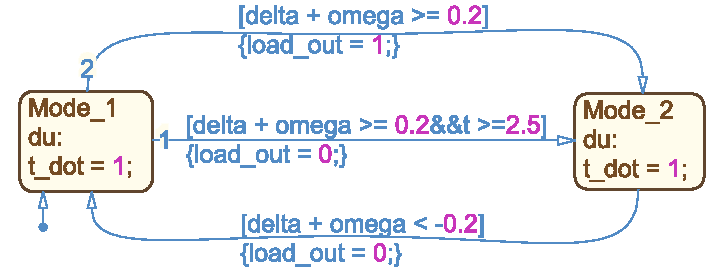
\includegraphics[width=0.42\textwidth]{image/smib_attack_model}%\vspace{1cm}
		%\includegraphics[trim = 17mm 85mm 17mm 0mm, clip, width=0.95\textwidth]{image/spectral_signal}%
	\caption{The Stateflow chart models the sliding-mode attack to the SMIB system.}%
	\figlabel{smib_attack_model}%
\end{figure}% 


\begin{figure*}[t!]%
	\centering%
    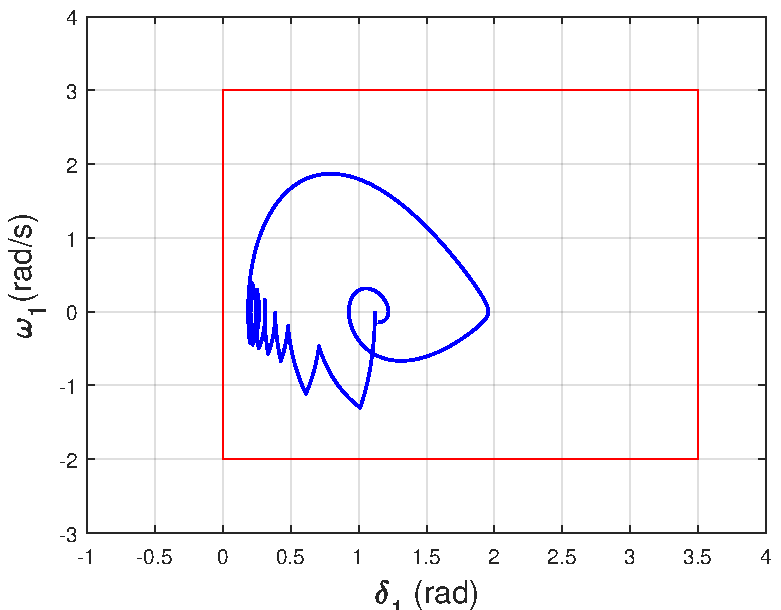
\includegraphics[width=0.31\textwidth]{image/normal}%\vspace{1cm}
		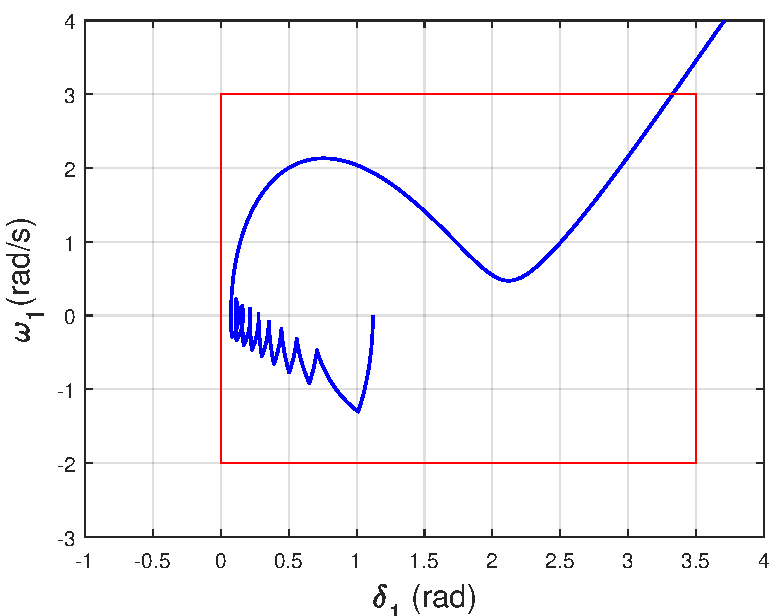
\includegraphics[width=0.31\textwidth]{image/counter}%
		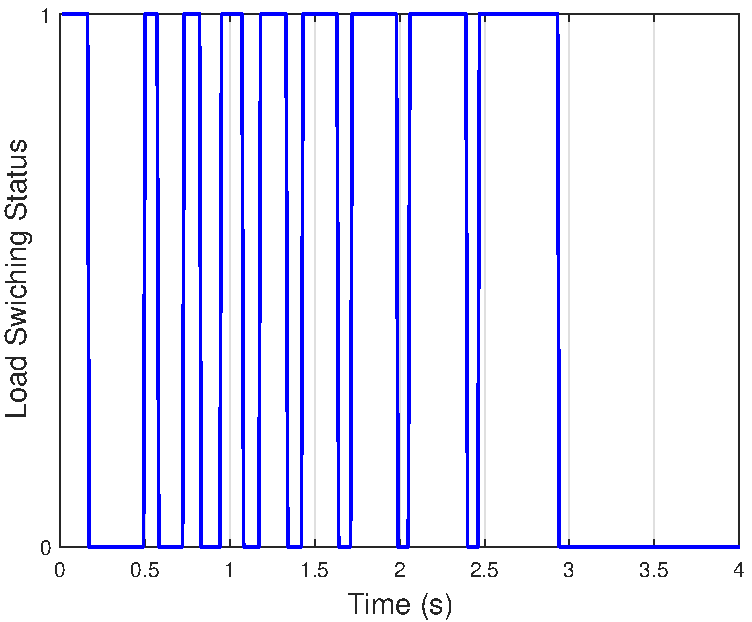
\includegraphics[width=0.3\textwidth]{image/load_v2}%
		%\includegraphics[trim = 17mm 85mm 17mm 0mm, clip, width=0.95\textwidth]{image/spectral_signal}%
	\caption{From left to right: 1) the stable system trajectory without an attack, 2) the counterexample represents the unstable system trajectory under the sliding-mode attack, and 3) the status of a circuit breaker during the attack, where 0 and 1 represent the disconnection and connection of the load $P_L$, respectively.}%
	\figlabel{smib_result}%
\end{figure*}% 

\vspace{0.5em}
\noindent
{\bf Resilient Pattern for SMIB Model.} 
As a sliding-mode attack is constructed based on switching back-and-forth the circuit breaker quickly to trap the system inside the sliding surface before guiding its state variables evolving outside the stability boundary, a potential strategy to mitigate such an attack is to increase the minimum switching time of the circuit breakers. Indeed, the designer can repair the original model by including a minimum dwell time in each mode of the system to prevent rapid switching.~\figref{smib_code} shows a resilient pattern written as a HATL script that introduces the \emph{clock} variable as a timer, and the switching time relies on the value of $\theta$.

\begin{figure}[!t]%frame=none,
\begin{lstlisting}[basicstyle=\ttfamily\footnotesize, numbers=none]
model = getModelByName("SMIB") # retrieve the plant model
	
# start a transformation  
addParam(model,"theta") # add a new parameter theta
addLocalVar(model,"clock") # add a clock variable
	
formode m = model.Mode {
    addFlow(m,"clock_dot = 1")
}

fortran t = model.Trans {
		# a transition only triggers after theta seconds
    addGuardLabel(t,"&&","clock > theta"); 
		# reset a clock after each transition
    addResetLabel(t,"clock = 0"); 
}
# end of the transformation
\end{lstlisting}
\caption{A dwell-time resilient pattern for the SMIB system.}%
\figlabel{smib_code}%
	%\vspace{-0.5em}%
\end{figure}


\begin{figure}[t!]%
	\centering%
    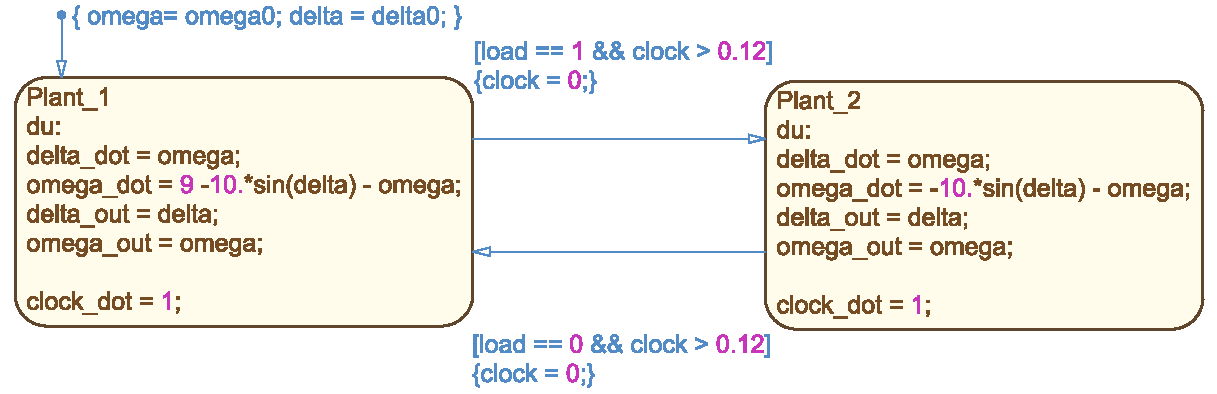
\includegraphics[width=0.48\textwidth]{image/smib_plant_model_res}%\vspace{1cm}
		%\includegraphics[trim = 17mm 85mm 17mm 0mm, clip, width=0.95\textwidth]{image/spectral_signal}%
	\caption{The resilient SMIB model with a synthesized dwell-time.}%
	\figlabel{smib_plant_model_res}%
\end{figure}% 

\vspace{0.5em}
\noindent
{\bf Resilient SMIB Model.} Given a resilient pattern shown in ~\figref{smib_code}, the model transformation of \toolreaffirm will convert the model to a new version that integrates the dwell-time pattern with the unknown parameter $\theta$.
%
Then, the model synthesis of \toolreaffirm calls Breach to search for the best (\ie minimum) value of $\theta$ over and the range of $[0, 1]$ that ensures the final model satisfies the STL \formref{smib_stl} under the sliding-mode attack. The final (resilient) model is shown in~\figref{smib_plant_model_res}, where the synthesized value of $\theta$ equals to $0.12$. As a result, the resilient model is stable, and its simulation trajectories contain within a red box, similar to the most left subfigure shown in \figref{smib_result}.


